%%%%%%%%%%%%%%%%%%%%%%%%%%%%%%%%%%%%%%%%%%%%%%%%%%%%%%%
% SEZIONE 6 — INTESTAZIONE + TESTO INTRODUTTIVO
%%%%%%%%%%%%%%%%%%%%%%%%%%%%%%%%%%%%%%%%%%%%%%%%%%%%%%%
\section{Risultati sperimentali}
\label{sec:06_risultati}

\epigraph{
    In God we trust; all others must bring data.
}{W. Edwards Deming}

In questo capitolo saranno presentati i risultati sperimentali ottenuti con PRISMA. Nel Paragrafo~\ref{subsec:setup} sarà descritta l'infrastruttura hardware e software utilizzata per gli esperimenti, con particolare attenzione alle motivazioni architetturali e di privacy che hanno guidato la scelta di una piattaforma di elaborazione interamente locale. Nel Paragrafo~\ref{subsec:feature_extraction_results} saranno analizzate le feature estratte dallo Sparse Autoencoder sul dominio scientifico, illustrandone le proprietà attraverso esempi concreti e discutendo l'organizzazione in famiglie semantiche gerarchiche. Infine, nel Paragrafo~\ref{subsec:effective_rank_results} sarà presentata l'analisi quantitativa dell'Effective Rank, che misura la dimensionalità effettiva dello spazio delle attivazioni al variare dell'expansion factor.

\newpage

%%%%%%%%%%%%%%%%%%%%%%%%%%%%%%%%%%%%%%%%%%%%%%%%%%%%%%%
% SUBSECTION: SETUP SPERIMENTALE
%%%%%%%%%%%%%%%%%%%%%%%%%%%%%%%%%%%%%%%%%%%%%%%%%%%%%%%
\subsection{Setup sperimentale}
\label{subsec:setup}
Prima di presentare i risultati ottenuti con PRISMA, è necessario descrivere l'infrastruttura hardware e software su cui sono stati condotti gli esperimenti. La scelta della piattaforma non è stata casuale: l'addestramento di Sparse Autoencoder e l'esecuzione di Large Language Models per l'interpretazione automatica delle feature richiedono risorse computazionali significative, in particolare per quanto riguarda la memoria disponibile. 
Inoltre, la natura sensibile dei dati trattati, vale a dire cartelle cliniche pediatriche fornite da 
% ****** MC: Sostituirei la frase qua sopra con ...
% Inoltre, i testi trattati, in particolare le cartelle cliniche pediatriche fornite da
Pedianet\footnote{Pedianet (\url{https://pedianet.it}) è una rete di ricerca che raccoglie dati clinici da pediatri di libera scelta italiani, 
costituendo uno dei più ampi database di medicina generale pediatrica in Europa.
% ****** MC: modificherei la riga qua sopra in
% gestisce uno dei più ampi database di medicina generale pediatrica in Europa
}, 
ha imposto 
% ****** MC: sostituirei la riga qua sopra con
% per quanto anonimizzate o prive di dati sensibili, tuttavia sono soggette a 
vincoli stringenti sulla localizzazione dell'elaborazione. PRISMA è stato infatti utilizzato anche per finalità di analisi su tali dati clinici; i relativi risultati non sono tuttavia riportati nella presente tesi, in quanto protetti da accordo di riservatezza (NDA). L'esigenza di un'infrastruttura di inferenza interamente locale, qui dettata dalla normativa sulla protezione dei dati sanitari, è peraltro comune a numerose realtà aziendali e istituzionali che trattano dati sensibili.
\subsubsection{Infrastruttura hardware}
\label{subsubsec:hardware}
Gli esperimenti sono stati condotti su un \textbf{Mac Studio} equipaggiato con chip \textbf{Apple M3 Ultra}
e 
% ****** MC: sostituirei con
%, dotato di Neural Engine e GPU per velocizzare algoritmi di Intelligenza Artificiale e calcolo matematico,
\textbf{512 GB} di memoria unificata. La Tabella~\ref{tab:hardware_specs} riassume le specifiche tecniche della macchina.

\begin{table}[htbp]
    \centering
    \caption{Specifiche hardware della macchina utilizzata per gli esperimenti.}
    \label{tab:hardware_specs}
    \begin{tabular}{@{}ll@{}}
        \toprule
        \textbf{Componente} & \textbf{Specifica} \\
        \midrule
        Modello & Mac Studio (Mac15,14) \\
        Chip & Apple M3 Ultra \\
        Core CPU & 32 (24 performance + 8 efficiency) \\
        Core GPU & 80 \\
        Neural Engine & 32 core \\
        Memoria unificata & 512 GB \\
        Bandwidth memoria & 819 GB/s \\
        \bottomrule
    \end{tabular}
\end{table}

La scelta di questa piattaforma è motivata da due fattori: una caratteristica architetturale distintiva dei chip Apple Silicon e un requisito di privacy imposto dalla natura dei dati.

\paragraph{La Unified Memory Architecture.}
A differenza delle architetture tradizionali, dove CPU e GPU dispongono di memorie separate (RAM di sistema e VRAM dedicata), nei chip Apple Silicon tutti i componenti computazionali, vale a dire CPU, GPU e Neural Engine, condividono lo stesso pool di memoria fisica. Questa architettura, denominata \textbf{Unified Memory Architecture} (UMA), elimina un collo di bottiglia fondamentale nel deep learning: il trasferimento dati tra CPU e GPU.

\begin{figure}[htbp]
    \centering
    \begin{tikzpicture}[
        scale=0.95,
        block/.style={draw, rectangle, rounded corners=4pt, minimum height=1.4cm, minimum width=2.8cm, font=\small, fill=#1, drop shadow={opacity=0.15}},
        memory/.style={draw, rectangle, rounded corners=6pt, minimum height=1.6cm, minimum width=11cm, font=\small\bfseries, fill=green!15, drop shadow={opacity=0.2}},
        arrow/.style={->, thick, gray!60},
        biarrow/.style={<->, very thick, green!50!black}
    ]
        
        % Contenitore chip (sfondo)
        \fill[gray!8, rounded corners=10pt] (-6, -0.5) rectangle (6, 4.2);
        \draw[thick, rounded corners=10pt, gray!40] (-6, -0.5) rectangle (6, 4.2);
        
        % Titolo chip
        \node[font=\normalsize\bfseries, gray!70] at (0, 3.7) {Apple M3 Ultra SoC};
        
        % CPU block
        \node[block=blue!25] (cpu) at (-3.5, 1.9) {
            \begin{tabular}{c}
                \textbf{CPU} \\
                \scriptsize 24 Performance \\
                \scriptsize 8 Efficiency
            \end{tabular}
        };
        
        % GPU block
        \node[block=orange!25] (gpu) at (0, 1.9) {
            \begin{tabular}{c}
                \textbf{GPU} \\
                \scriptsize 80 cores \\
                \scriptsize Ray Tracing
            \end{tabular}
        };
        
        % Neural Engine block
        \node[block=violet!25] (ne) at (3.5, 1.9) {
            \begin{tabular}{c}
                \textbf{Neural Engine} \\
                \scriptsize 32 cores \\
                \scriptsize 31 TOPS
            \end{tabular}
        };
        
        % Memory controller (barra)
        \fill[gray!20, rounded corners=3pt] (-5, 0) rectangle (5, 0.5);
        \draw[gray!50, rounded corners=3pt] (-5, 0) rectangle (5, 0.5);
        \node[font=\scriptsize\bfseries, gray!70] at (0, 0.25) {Memory Fabric · 819 GB/s};
        
        % Frecce dai componenti al memory controller
        \draw[arrow, line width=1.2pt] (cpu.south) -- ++(0, -0.35);
        \draw[arrow, line width=1.2pt] (gpu.south) -- ++(0, -0.35);
        \draw[arrow, line width=1.2pt] (ne.south) -- ++(0, -0.35);
        
        % Unified Memory (sotto)
        \node[memory] (mem) at (0, -1.7) {Unified Memory — 512 GB LPDDR5};
        
        % Freccia bidirezionale memory controller <-> memoria
        \draw[biarrow, line width=2pt] (0, -0.1) -- (0, -0.9);
        
        % Annotazioni software (fuori dal chip)
        \node[font=\scriptsize, blue!60!black, align=center] (ann1) at (-3.5, -3.5) {PyTorch MPS\\SAE Training};
        \draw[->, blue!50, thick, dashed] (ann1.north) -- (-3.5, -2.5);
        
        \node[font=\scriptsize, orange!70!black, align=center] (ann2) at (0, -3.5) {BERT\\Embeddings};
        \draw[->, orange!50, thick, dashed] (ann2.north) -- (0, -2.5);
        
        \node[font=\scriptsize, violet!60!black, align=center] (ann3) at (3.5, -3.5) {Ollama\\LLM Interpreter};
        \draw[->, violet!50, thick, dashed] (ann3.north) -- (3.5, -2.5);
        
        % Nota zero-copy
        \node[draw, rounded corners=3pt, fill=yellow!10, font=\scriptsize, inner sep=4pt] at (0, -4.5) {Zero-copy: tutti i componenti accedono agli stessi dati senza trasferimenti};
        
    \end{tikzpicture}
    \caption{Architettura del chip Apple M3 Ultra con Unified Memory Architecture (UMA). I tre componenti computazionali, vale a dire CPU, GPU e Neural Engine, condividono lo stesso pool di 512 GB di memoria LPDDR5, accessibile attraverso un memory fabric con bandwidth aggregato di 819 GB/s. Il \textbf{Neural Engine} è un acceleratore hardware dedicato alle operazioni di machine learning (moltiplicazioni matriciali, convoluzioni), capace di 31 trilioni di operazioni al secondo (TOPS); viene sfruttato da Ollama per accelerare l'inferenza dei Large Language Models utilizzati come interpreti delle feature. L'architettura elimina i trasferimenti CPU-GPU tipici dei sistemi con memorie separate, abilitando workflow che alternano preprocessing (CPU), training (GPU) e inferenza LLM (Neural Engine) sugli stessi dati.}
    \label{fig:m3_ultra_architecture}
\end{figure}

\paragraph{Il collo di bottiglia nelle architetture tradizionali.}
Per comprendere il vantaggio della UMA, è utile considerare come funzionano le architetture convenzionali. In un sistema con CPU e GPU discrete, i due processori dispongono di memorie fisicamente separate: la RAM di sistema (accessibile alla CPU) e la VRAM (accessibile alla GPU). Quando si addestra una rete neurale, i dati devono essere copiati dalla RAM alla VRAM prima di ogni operazione su GPU, e i risultati devono essere copiati indietro per l'elaborazione su CPU.

Il canale di comunicazione tra CPU e GPU è 
di solito % ****** aggiunto da MC
il bus \textbf{PCIe} (Peripheral Component Interconnect Express). Anche nelle configurazioni più recenti, 
%il
la % ****** Modificato da MC 
bandwidth di questo canale 
%è
ha % ****** modificato da MC
ordini di grandezza inferiore a quello della memoria locale:

\begin{table}[htbp]
    \centering
    \caption{Confronto della memory bandwidth tra architetture. La bandwidth misura quanti dati possono essere trasferiti al secondo tra memoria e processori, un fattore critico per workload memory-bound come l'inferenza di LLM.}
    \label{tab:bandwidth_comparison}
    \begin{tabular}{@{}lrl@{}}
        \toprule
        \textbf{Interfaccia} & \textbf{Bandwidth} & \textbf{Note} \\
        \midrule
        PCIe 4.0 x16 & 32 GB/s & Standard attuale per GPU \\
        PCIe 5.0 x16 & 64 GB/s & Ultima generazione \\
        \midrule
        NVIDIA RTX 4090 (VRAM) & 1.008 GB/s & Memoria locale GPU \\
        NVIDIA A100 80GB (VRAM) & 2.039 GB/s & GPU professionale \\
        \midrule
        \textbf{Apple M3 Ultra (UMA)} & \textbf{819 GB/s} & Memoria unificata \\
        \bottomrule
    \end{tabular}
\end{table}

Il problema emerge chiaramente: anche se la VRAM di una GPU NVIDIA ha una bandwidth elevatissima (1--2 TB/s), i dati devono prima \textit{attraversare} il bus PCIe, che è 15--30 volte più lento. Per workload che richiedono frequenti trasferimenti CPU-GPU, come l'addestramento di autoencoder con preprocessing su CPU, questo diventa il collo di bottiglia dominante.


\begin{notebox}
\textbf{Analogia: il magazzino e la porta}\\[0.5em]
La memory bandwidth può essere compresa con un'analogia. Si immagini la memoria come un magazzino e i processori (CPU/GPU) come operai che devono lavorare i materiali:
\begin{itemize}
    \item La \textbf{capacità della memoria} (512 GB) corrisponde alla dimensione del magazzino
    \item Il \textbf{memory bandwidth} (819 GB/s) corrisponde alla larghezza della porta
\end{itemize}
Un magazzino enorme con una porta stretta costringe gli operai ad aspettare i materiali. Nelle architetture tradizionali, la ``porta'' tra CPU e GPU (il bus PCIe) è molto più stretta della ``porta'' verso le rispettive memorie locali. Con la 
%UMA, 
Unified Memory Architecture,
CPU e GPU condividono lo stesso  
% magazzino e la stessa porta, larga 819 GB/s.
% ****** Ho sostituito la riga qua sopra con la seguente
magazzino, non c'è porta di separazione tra i due ambienti, l'unica porta esistente è verso l'esterno (dischi, rete, etc.) ed ha una banda di 819 GB/s. 

\end{notebox}
Con la Unified Memory Architecture, questo collo di bottiglia scompare. Un tensore allocato in memoria è immediatamente accessibile sia dalla CPU che dalla GPU, senza alcuna copia (\textit{zero-copy}). Il bandwidth di 819 GB/s, 25 volte superiore a PCIe 4.0, è disponibile per \textit{tutti} i componenti simultaneamente.
\paragraph{Superamento dei limiti della VRAM.}
Il secondo vantaggio della UMA riguarda la capacità. Le GPU consumer più potenti (NVIDIA RTX 4090) dispongono di 24 GB di VRAM; le GPU professionali (NVIDIA A100) arrivano a 80 GB. Con 512 GB di memoria unificata, il Mac Studio può caricare modelli che eccederebbero la VRAM di qualsiasi GPU singola.
Questo è particolarmente rilevante per i Large Language Models. DeepSeek-V3~\parencite{deepseekai2024deepseekv3}, con 671 miliardi di parametri, richiede circa 400 GB di memoria anche in formato quantizzato\footnote{La quantizzazione riduce la precisione dei pesi (ad esempio da 16 bit a 4 bit) per diminuire l'occupazione di memoria. Una trattazione dettagliata è riportata in Appendice~\ref{app:quantization}.}. Sul Mac Studio utilizzato, è possibile eseguire questo modello interamente in memoria, senza ricorrere a tecniche di \textit{offloading} su disco o a cluster multi-GPU, opzioni che introdurrebbero latenza significativa e complessità architetturale.
\paragraph{Metal Performance Shaders (MPS).}
PyTorch supporta l'accelerazione GPU su Apple Silicon attraverso il backend MPS (\texttt{torch.device("mps")}). Questo permette di sfruttare gli 80 core GPU del M3 Ultra per l'addestramento degli Sparse Autoencoder, ottenendo prestazioni significativamente superiori rispetto all'esecuzione su sola CPU.
\paragraph{Requisiti di privacy: elaborazione locale dei dati clinici.}
Oltre ai vantaggi prestazionali, la scelta di un'infrastruttura locale è stata dettata da un requisito non negoziabile: 
% ****** MC, ho aggiunto la riga seguente
utilizzare un ambiente di elaborazione in grado di garantire
la \textbf{privacy dei dati}. Come anticipato, PRISMA è stato impiegato anche per l'analisi di cartelle cliniche pediatriche fornite da Pedianet che, sebbene anonimizzate, contengono informazioni 
%sensibili 
% ****** Ho modificato la riga sopra nel modo seguente
sanitarie
non trasmissibili a servizi cloud esterni.
%
%L'
% ****** MC, ho modificato la riga sopra nel modo seguente
E' stato escluso a priori 
l'utilizzo di API cloud per l'interpretazione delle feature, ad esempio inviando i testi attivanti a GPT-4~\parencite{openai2023gpt4} o Claude~\parencite{anthropic2024claude}
%, avrebbe 
Ciò avrebbe
comportato il trasferimento di dati clinici su server di terze parti, una pratica incompatibile con le normative sulla protezione dei dati sanitari e con i principi etici della ricerca medica. La disponibilità di 512 GB di memoria unificata ha permesso di eseguire \textit{localmente} modelli linguistici di grande scala, quali DeepSeek~\parencite{deepseekai2024deepseekv3}, Llama~\parencite{touvron2023llama} e Qwen~\parencite{bai2023qwen}, attraverso 
% ****** MC, ho aggiunto la riga
l'infrastruttura
Ollama, garantendo che nessun dato clinico lasciasse mai la macchina.
Questa configurazione, vale a dire un'elaborazione interamente on-premise con hardware sufficientemente potente da eseguire LLM di frontiera, rappresenta attualmente una soluzione rara nel panorama del deep learning, dove la maggior parte dei workflow 
% assume 
presuppone
l'accesso a risorse cloud. Il Mac Studio con M3 Ultra e 512 GB di memoria è una delle poche piattaforme consumer che rende possibile questo approccio.


%%%%%%%%%%%%%%%%%%%%%%%%%%%%%%%%%%%%%%%%%%%%%%%%%%%%%%%
% SUBSECTION: ESTRAZIONE E ORGANIZZAZIONE DELLE FEATURE
%%%%%%%%%%%%%%%%%%%%%%%%%%%%%%%%%%%%%%%%%%%%%%%%%%%%%%%
\subsection{Estrazione e organizzazione delle feature}
\label{subsec:feature_extraction_results}

\subsubsection{Dataset e pipeline di embedding}
\label{subsubsec:dataset_embedding}
Il corpus utilizzato per gli esperimenti sul dominio scientifico è costituito da circa \textbf{2,5 milioni di abstract} estratti dal dataset \texttt{common-pile/arxiv\_abstracts}, disponibile pubblicamente su HuggingFace\footnote{\url{https://huggingface.co/datasets/common-pile/arxiv_abstracts}}. Il dataset copre l'intero spettro disciplinare di arXiv, dalla fisica teorica all'informatica, dalla matematica alla biologia quantitativa, offrendo un banco di prova ideale per valutare la capacità dei SAE di estrarre strutture semantiche da un dominio ad alta diversità concettuale.

Ciascun abstract è stato trasformato in un vettore denso di dimensione $d = 384$ tramite il modello \texttt{sentence-transformers/all-MiniLM-L6-v2}\footnote{\url{https://huggingface.co/sentence-transformers/all-MiniLM-L6-v2}}, un sentence encoder leggero basato su MiniLM~\parencite{wang2020minilm} che produce embedding ottimizzati per la similarità semantica a livello di frase. La scelta di questo modello, rispetto a encoder più pesanti come BERT-large~\parencite{devlin2018bert}, è motivata dal trade-off favorevole tra qualità delle rappresentazioni e costo computazionale: con 22 milioni di parametri e una dimensione di embedding di 384, \texttt{all-MiniLM-L6-v2} consente di processare milioni di documenti in tempi ragionevoli mantenendo prestazioni competitive sui benchmark di sentence similarity.

\subsubsection{Interpretazione automatica delle feature}
\label{subsubsec:feature_interpretation}
Lo Sparse Autoencoder addestrato sugli embedding del corpus arXiv ha prodotto uno spazio latente con migliaia di direzioni attive. Per rendere queste direzioni semanticamente leggibili, si è proceduto all'interpretazione automatica tramite un LLM locale, secondo la metodologia descritta nel Paragrafo~\ref{subsubsec:interpreter}.

Il modello utilizzato come interprete è \textbf{Gemma 3 27B}\footnote{\url{https://ollama.com/library/gemma3:27b}}, eseguito localmente tramite Ollama sulla macchina descritta nel Paragrafo~\ref{subsec:setup}. Per ciascuna feature, l'interprete ha ricevuto in input i testi con le attivazioni più alte (\textit{top activating contexts}) e i contro-esempi, producendo un'etichetta semantica in linguaggio naturale. Complessivamente, sono state interpretate con successo più di \textbf{4.000 feature}, ciascuna associata a una descrizione testuale del concetto che la direzione latente codifica.

Il processo di interpretazione su larga scala, vale a dire oltre 4.000 feature ciascuna richiedente un prompt con più esempi e una generazione di testo, ha beneficiato significativamente dei 512~GB di memoria unificata del Mac Studio, che hanno permesso di mantenere il modello da 27 miliardi di parametri interamente in memoria durante l'intera sessione di labelling.

\subsubsection{Esempio: Feature 5648 --- \textit{Time in physics}}
\label{subsubsec:feature_example}
Per illustrare concretamente il tipo di struttura estratta dal SAE, si esamini la \textbf{Feature 5648} del modello SAE \#10 (Figura~\ref{fig:feature_5648_label}). L'interprete Gemma 3 ha assegnato a questa feature la seguente etichetta semantica:
\begin{figure}[htbp]
    \centering
    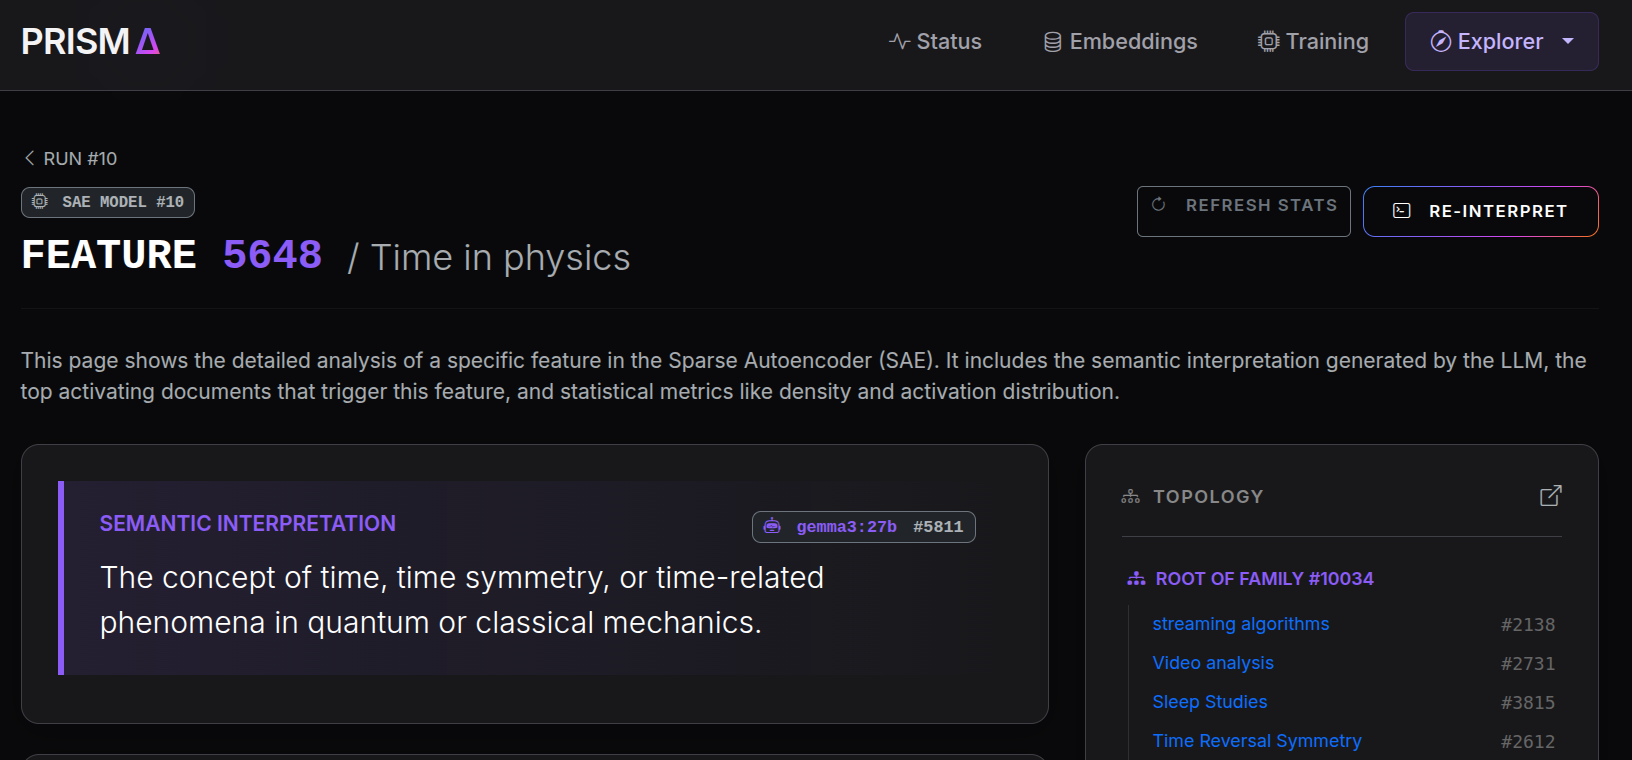
\includegraphics[width=\textwidth]{pictures/cap6/feature_5648_label.png}
    \caption{Descrizione della feature 5648 generata dal LLM interprete}
    \label{fig:feature_5648_label}
\end{figure}

\begin{figure}[htbp]
    \centering
    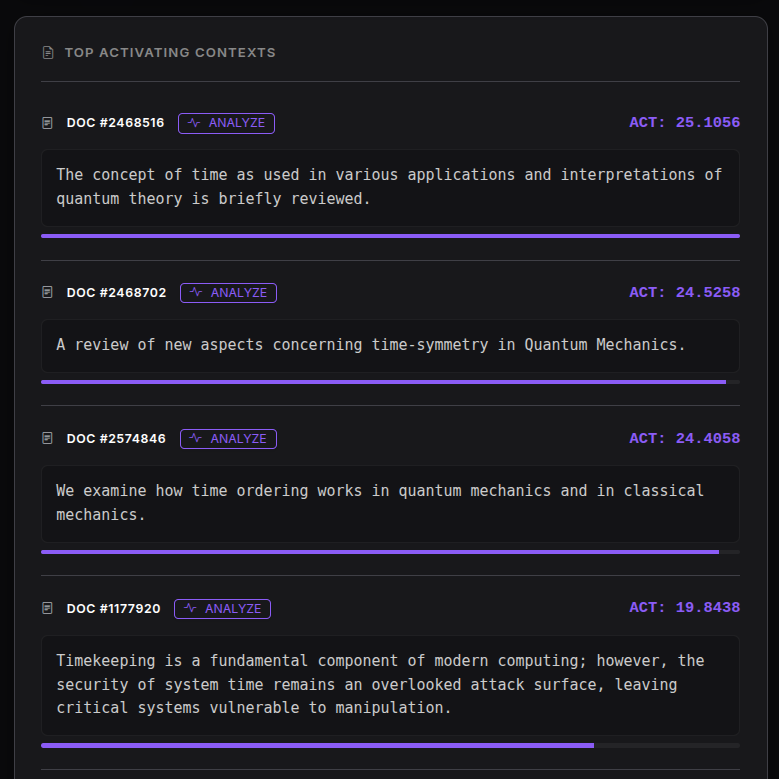
\includegraphics[width=\textwidth]{pictures/cap6/feature_5648_docs.png}
    \caption{Documenti che hanno maggiormente attivato il neurone associato alla feature 5648}
    \label{fig:feature_5648_docs}
\end{figure}

\begin{figure}[htbp]
    \centering
    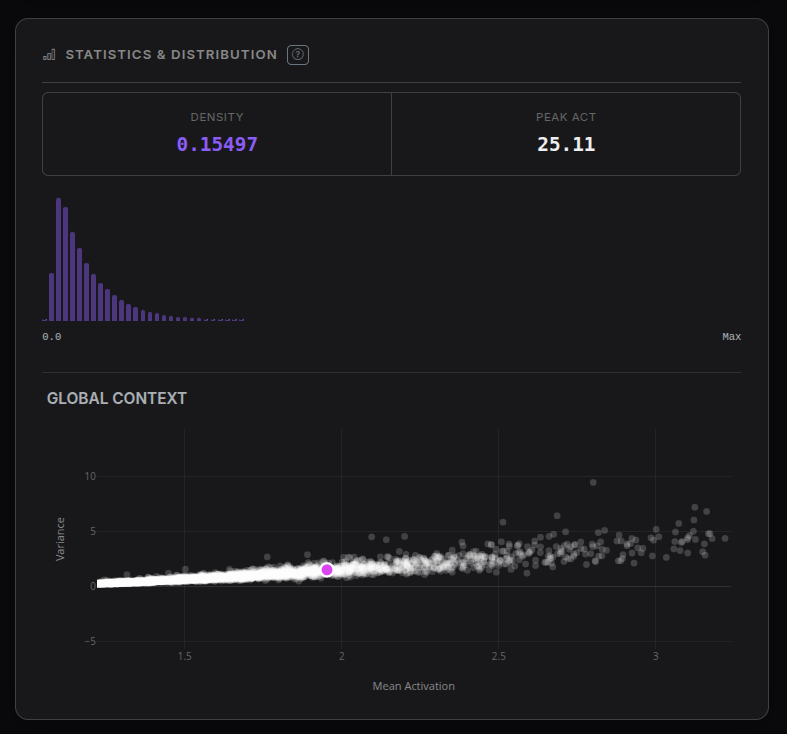
\includegraphics[width=\textwidth]{pictures/cap6/feature_5648_2.png}
    \caption{Posizionamento della feature 5648 nello scatter plot delle attivazioni su media e varianza delle intensità di attivazioni dei neuroni.}
    \label{fig:feature_5648_scatter}
\end{figure}


\begin{quote}
\textit{``The concept of time, time symmetry, or time-related phenomena in quantum or classical mechanics.''}
\end{quote}

\paragraph{Statistiche di attivazione.}
La feature presenta una \textbf{densità} di 0.155, indicando che si attiva su circa il 15,5\% dei documenti del corpus, un valore coerente con la pervasività del concetto di tempo nella letteratura fisica. L'\textbf{attivazione di picco} è 25.11, osservata su abstract che trattano esplicitamente la natura del tempo in meccanica quantistica.

\paragraph{Top activating contexts.}
I documenti che massimizzano l'attivazione della feature confermano la coerenza dell'interpretazione:

\begin{table}[htbp]
    \centering
    \caption{Top activating contexts per la Feature 5648 (\textit{Time in physics}).}
    \label{tab:feature_5648_top}
    \begin{tabular}{@{}clr@{}}
        \toprule
        \textbf{Doc ID} & \textbf{Abstract (estratto)} & \textbf{Attivazione} \\
        \midrule
        2468516 & \textit{The concept of time as used in various applications} & 25.11 \\
                & \textit{and interpretations of quantum theory [\ldots]} & \\
        2468702 & \textit{A review of new aspects concerning time-symmetry} & 24.53 \\
                & \textit{in Quantum Mechanics.} & \\
        2574846 & \textit{We examine how time ordering works in quantum} & 24.41 \\
                & \textit{mechanics and in classical mechanics.} & \\
        1177920 & \textit{Timekeeping is a fundamental component of modern} & 19.84 \\
                & \textit{computing [\ldots] security of system time [\ldots]} & \\
        2455750 & \textit{A very brief and popular account of the time} & 19.63 \\
                & \textit{machine problem.} & \\
        \bottomrule
    \end{tabular}
\end{table}

Si noti il gradiente di attivazione: i tre documenti con attivazione più alta ($>24$) trattano specificamente il tempo come concetto fondamentale in meccanica quantistica e classica. I documenti con attivazione più bassa ($\sim$19--20) riguardano il tempo in contesti adiacenti ma meno centrali, vale a dire la sicurezza del system time nei sistemi informatici e il problema divulgativo delle macchine del tempo. Questo gradiente mostra che la feature non è un semplice classificatore binario, ma codifica un \textit{grado di rilevanza} continuo rispetto al concetto.

\paragraph{Topologia e famiglia semantica.}
La Feature 5648 risulta essere la \textbf{radice} della \textbf{Famiglia \#10034}, una famiglia che raggruppa 47 feature children tra cui:

\begin{itemize}
    \item \textit{Time Reversal Symmetry} (\#2612)
    \item \textit{Event Modeling} (\#515)
    \item \textit{Sleep Studies} (\#3815)
    \item \textit{Video Analysis} (\#2731)
    \item \textit{Streaming Algorithms} (\#2138)
\end{itemize}

La struttura è coerente con la topologia a stella tipica delle feature families: il parent \textit{Time in physics} rappresenta il concetto temporale nella sua accezione più generale, mentre i children catturano specializzazioni, dalla simmetria temporale in fisica alle applicazioni computazionali che coinvolgono la dimensione temporale (streaming, video, modellazione di eventi).

\paragraph{Correlazioni.}
Le correlazioni nello spazio dei pesi (\textit{weight-space}, similarità tra vettori decoder) e nello spazio dei dati (\textit{co-attivazione}) offrono ulteriori conferme della coerenza semantica. Si ricordi che la matrice $S$ cattura la similarità geometrica tra le colonne del decoder, vale a dire feature che ``puntano'' in direzioni simili nello spazio degli embedding, mentre la matrice $D$ misura la co-occorrenza statistica sugli stessi documenti:

\begin{table}[htbp]
    \centering
    \caption{Correlazioni della Feature 5648 nello spazio dei pesi (S) e dei dati (D).}
    \label{tab:feature_5648_corr}
    \begin{tabular}{@{}llr@{}}
        \toprule
        \textbf{Tipo} & \textbf{Feature correlata} & \textbf{Correlazione} \\
        \midrule
        S & Mathematical Graph Theory & 0.21 \\
        S & Operator Theory & 0.20 \\
        S & Polynomial Time Algorithm & 0.18 \\
        S & Period Mappings & 0.18 \\
        \midrule
        D & Zero Modes & 0.23 \\
        D & Mathematical or Physics Research & 0.18 \\
        D & Quantum Mechanics & 0.17 \\
        D & Quantum Gravity & 0.15 \\
        D & Hadron Physics & 0.15 \\
        \bottomrule
    \end{tabular}
\end{table}

Le correlazioni di co-attivazione (D) sono particolarmente informative: la feature \textit{Time in physics} tende a co-attivarsi con \textit{Quantum Mechanics}, \textit{Quantum Gravity} e \textit{Hadron Physics}, vale a dire esattamente le aree della fisica in cui il concetto di tempo ha un ruolo fondamentale. La correlazione con \textit{Zero Modes} riflette la connessione tra simmetrie temporali e modi zero nelle teorie di gauge. Le correlazioni nello spazio dei pesi (S), invece, rivelano prossimità geometriche nel decoder con feature di natura più matematica (\textit{Operator Theory}, \textit{Graph Theory}), suggerendo che il SAE ha appreso una regione dello spazio latente dove strutture temporali e strutture algebriche astratte condividono direzioni simili.

\subsubsection{Esempio: Feature 1140 --- \textit{Ising model}}
\label{subsubsec:feature_example_ising}
Come secondo esempio, si consideri la \textbf{Feature 1140}, che illustra un caso complementare rispetto alla precedente: una feature altamente \textit{specifica}, con densità molto bassa e semantica circoscritta a un singolo modello teorico. L'interprete Gemma 3 ha prodotto l'etichetta:

\begin{quote}
\textit{``Two-dimensional Ising model statistical physics.''}
\end{quote}

\paragraph{Statistiche di attivazione.}
La densità di questa feature è \textbf{0.00772}, quasi venti volte inferiore a quella della Feature 5648. Ciò significa che la feature si attiva su meno dell'1\% del corpus, coerentemente con il fatto che il modello di Ising bidimensionale è un argomento di nicchia anche all'interno della fisica teorica. L'attivazione di picco è 24.68, comparabile a quella della Feature 5648, indicando che quando la feature si attiva lo fa con intensità elevata: il SAE ha appreso una direzione latente \textit{stretta ma profonda}.

\paragraph{Top activating contexts.}
I documenti con attivazione massima confermano la specificità dell'interpretazione:

\begin{table}[htbp]
    \centering
    \caption{Top activating contexts per la Feature 1140 (\textit{Ising model}).}
    \label{tab:feature_1140_top}
    \begin{tabular}{@{}clr@{}}
        \toprule
        \textbf{Doc ID} & \textbf{Abstract (estratto)} & \textbf{Attivazione} \\
        \midrule
        479389  & \textit{One more solution of 2D Ising model is found} & 24.68 \\
        382080  & \textit{We show that the center of mass of Ising vectors} & 16.58 \\
                & \textit{that obey some simple constraints [\ldots]} & \\
        2315193 & \textit{The partition function and magnetization equations} & 14.58 \\
                & \textit{are derived for the 2D nearest neighbour Ising models [\ldots]} & \\
        1597255 & \textit{The correlation functions of the Z-invariant Ising} & 13.95 \\
                & \textit{model [\ldots] Vertex Operators language [\ldots]} & \\
        481058  & \textit{The partition function of 2D nearest neighbour Ising} & 13.79 \\
                & \textit{models in a non-zero magnetic field [\ldots]} & \\
        \bottomrule
    \end{tabular}
\end{table}

A differenza della Feature 5648, qui il gradiente di attivazione è più ripido: il documento di picco (24.68) è seguito da un salto a 16.58, poi valori compressi tra 13 e 15. Questo profilo è tipico delle feature \textit{monosemantiche strette}: il concetto codificato è sufficientemente specifico da generare un'attivazione massima solo quando l'abstract riguarda \textit{esattamente} il modello di Ising 2D, con decadimento rapido per trattazioni tangenziali.

\paragraph{Topologia e famiglia semantica.}
A differenza della Feature 5648, che è la radice di una famiglia, la Feature 1140 è un \textbf{child} della Feature \#1734 (\textit{Zero Modes}). Questa relazione gerarchica è fisicamente sensata: i modi zero emergono naturalmente nello studio delle transizioni di fase del modello di Ising, in particolare in connessione con la simmetria $\mathbb{Z}_2$ e i modi di Goldstone.

\paragraph{Correlazioni.}
\begin{table}[htbp]
    \centering
    \caption{Correlazioni della Feature 1140 nello spazio dei pesi (S) e dei dati (D).}
    \label{tab:feature_1140_corr}
    \begin{tabular}{@{}llr@{}}
        \toprule
        \textbf{Tipo} & \textbf{Feature correlata} & \textbf{Correlazione} \\
        \midrule
        S & Baryon/Boson Spectroscopy & 0.54 \\
        S & Wasserstein Distance & 0.35 \\
        S & Amenability & 0.33 \\
        S & Besov Spaces & 0.33 \\
        S & Black Hole Entropy and Thermodynamics & 0.29 \\
        \midrule
        D & Zero Modes & 0.42 \\
        D & Quantum Spin & 0.38 \\
        D & Phase Transitions & 0.33 \\
        D & Thermal Physics & 0.33 \\
        D & Quantum Mechanics & 0.32 \\
        D & Magnetic Fields and Materials & 0.31 \\
        \bottomrule
    \end{tabular}
\end{table}

% ****** Mirko sei arrivato qui 

Le correlazioni di co-attivazione (D) disegnano una mappa concettuale notevolmente precisa del modello di Ising: \textit{Quantum Spin}, \textit{Phase Transitions}, \textit{Thermal Physics} e \textit{Magnetic Fields and Materials} sono esattamente i pilastri concettuali su cui si fonda il modello, vale a dire spin discreti su reticolo, transizioni di fase ferromagnetiche, termodinamica statistica, interazioni magnetiche. La correlazione più alta con \textit{Zero Modes} (0.42) è coerente con la relazione parent-child nella topologia delle famiglie.

Le correlazioni nello spazio dei pesi (S) rivelano una struttura più sorprendente: la correlazione elevata con \textit{Baryon/Boson Spectroscopy} (0.54) suggerisce che il decoder ha appreso una prossimità geometrica tra il modello di Ising e la spettroscopia delle particelle, due domini apparentemente distanti ma accomunati dal formalismo della meccanica statistica e delle teorie di campo su reticolo.

La Feature 5648 è un concetto \textit{parent}, ampio, pervasivo, radice di una famiglia estesa, mentre la Feature 1140 è un concetto \textit{child}, specifico, raro, subordinato a un parent. Entrambe, tuttavia, mostrano attivazioni di picco comparabili ($\sim$25), indicando che il SAE assegna intensità elevata sia a concetti generali sia a concetti specifici quando l'input è altamente pertinente. Questa capacità di operare simultaneamente a livelli di granularità diversi, dal macro-concetto alla sotto-specializzazione, è una proprietà centrale della rappresentazione sparsa overcomplete.

\subsubsection{Feature families nel dominio scientifico}
\label{subsubsec:scientific_features}
Gli esempi delle Feature 5648 e 1140 sono rappresentativi di un pattern più generale. L'algoritmo di clustering gerarchico descritto nel Paragrafo~\ref{subsubsec:feature_families}, applicato alle oltre 4.000 feature interpretate, ha identificato \textbf{590 feature families}. Ciascuna famiglia è organizzata attorno a un \textbf{parent}, una feature a semantica ampia che funge da radice, e un insieme di \textbf{children}, feature più specifiche che ne rappresentano specializzazioni concettuali.

\paragraph{Caso di studio: Famiglia \#10034 --- \textit{Time in physics}.}
La Famiglia \#10034, il cui parent è la Feature 5648 (\textit{Time in physics}), offre un esempio paradigmatico di questa organizzazione. Come mostrato nella Figura~\ref{fig:time_physics_list}, la famiglia raggruppa 47 children che coprono un ventaglio di specializzazioni del concetto di tempo: dalla \textit{Time Reversal Symmetry} (\#2612) alla \textit{Special Relativity} (\#4811), dai \textit{Quantum Clocks} (\#4456) alle \textit{Particle Lifetimes} (\#914), fino ad applicazioni computazionali come gli \textit{Streaming Algorithms} (\#2138) e la \textit{Sliding Window Analysis} (\#2970). Compaiono anche specializzazioni inattese ma semanticamente coerenti: \textit{Option Pricing} (\#2639), dove il tempo è la variabile fondamentale nei modelli di Black-Scholes, e \textit{Biological Aging} (\#5060), dove il tempo è l'asse lungo cui si misurano i processi di senescenza.

\begin{figure}[htbp]
    \centering
    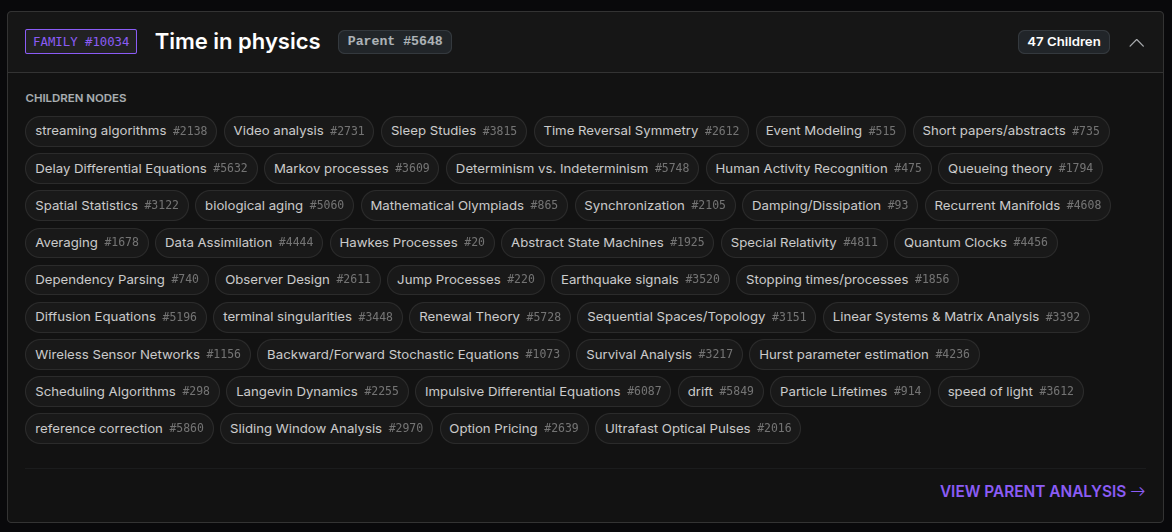
\includegraphics[width=\textwidth]{pictures/cap6/time_in_physics_list.png}
    \caption{Famiglia \#10034 (\textit{Time in physics}): lista completa dei 47 children nodes. Ogni chip riporta l'etichetta semantica e l'indice della feature. Si noti la diversità disciplinare dei children, dalla fisica fondamentale (\textit{Special Relativity}, \textit{Quantum Clocks}) alla matematica applicata (\textit{Renewal Theory}, \textit{Diffusion Equations}) fino a domini applicativi (\textit{Option Pricing}, \textit{Scheduling Algorithms}), tutti accomunati dalla centralità del concetto di tempo.}
    \label{fig:time_physics_list}
\end{figure}

La Figura~\ref{fig:time_physics_graph} mostra la stessa famiglia nella visualizzazione a grafo dell'Explorer di PRISMA. La topologia a stella è immediatamente riconoscibile: il nodo centrale azzurro (\textit{Time in physics}) irradia connessioni verso i children (nodi viola), che a loro volta possono essere connessi a feature di famiglie adiacenti (\textit{Quantum States}, \textit{Cosmic Dust}, \textit{Algebraic Structures}, ecc.), creando un tessuto di relazioni inter-famiglia che riflette la struttura interdisciplinare della ricerca scientifica.

\begin{figure}[htbp]
    \centering
    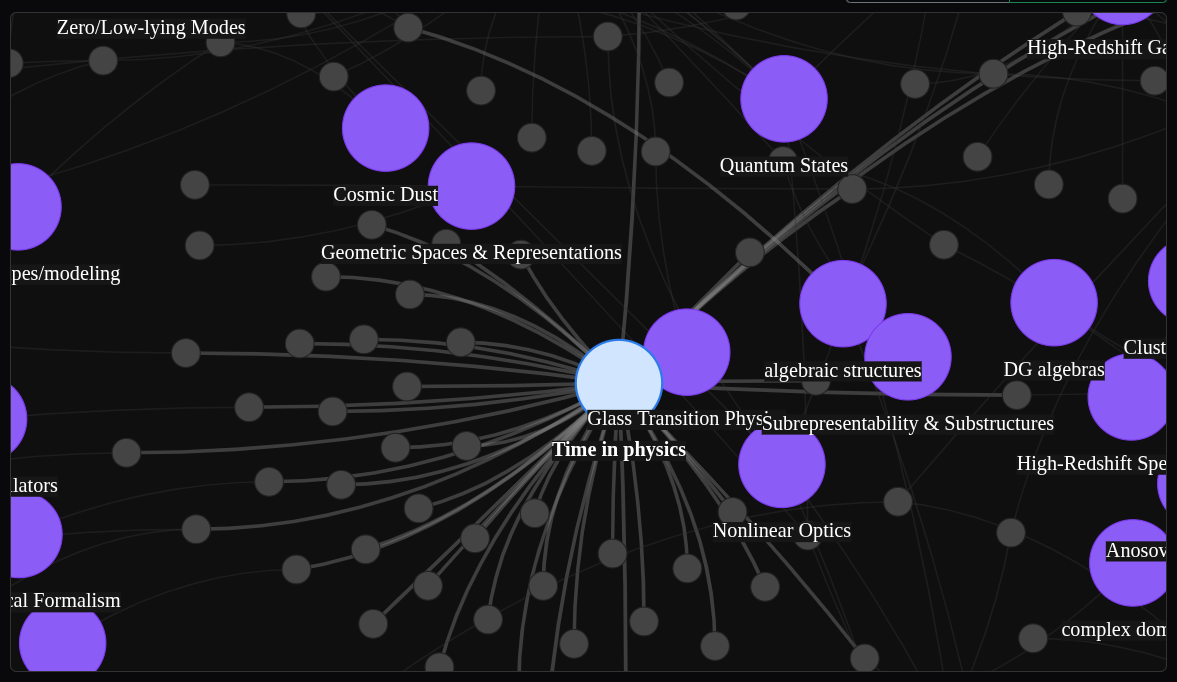
\includegraphics[width=\textwidth]{pictures/cap6/time_in_physics_graph.png}
    \caption{Visualizzazione a grafo della Famiglia \#10034 nell'Explorer di PRISMA. Il nodo centrale azzurro è il parent \textit{Time in physics}; i nodi viola sono i children e le feature correlate di famiglie adiacenti. La topologia a stella, tipica delle feature families, emerge chiaramente: il parent funge da nodo concettuale centrale, mentre i children raramente sono connessi direttamente tra loro.}
    \label{fig:time_physics_graph}
\end{figure}

\subsubsection{Le 590 famiglie come assi di una rappresentazione}
\label{subsubsec:families_as_axes}
L'analisi delle 590 famiglie rivela che la struttura a stella osservata per \textit{Time in physics} non è un caso isolato, ma un pattern ricorrente. Le famiglie mappano in modo coerente le aree disciplinari e le metodologie della ricerca scientifica, dai sottocampi del machine learning alla fisica delle particelle. Questi risultati sono consistenti con quelli riportati in~\parencite{oneill2024disentangling}, confermando che la metodologia degli Sparse Autoencoder produce feature semanticamente interpretabili anche quando applicata con modelli di embedding e infrastrutture diverse.
L'esistenza di 590 feature families suggerisce una prospettiva interessante. Se ciascuna famiglia cattura un asse concettuale distinto, come \textit{tempo}, \textit{modello di Ising}, \textit{sintomi respiratori} o \textit{ottimizzazione}, allora le 590 famiglie potrebbero potenzialmente essere considerate come gli \textbf{assi indipendenti} di una rappresentazione semantica compressa. In questa lettura, il SAE non si limiterebbe a estrarre feature isolate, ma rivelerebbe una \textit{base concettuale} del dominio: un insieme di direzioni semantiche lungo le quali varia il contenuto del corpus.
Tuttavia, questa interpretazione solleva una domanda quantitativa: le 590 famiglie sono davvero indipendenti? O esistono correlazioni residue tra famiglie, ad esempio la famiglia \textit{Thermal Physics} potrebbe co-attivarsi sistematicamente con la famiglia \textit{Phase Transitions}, che riducono i gradi di libertà effettivi al di sotto di 590? In altri termini: qual è la \textbf{dimensionalità effettiva} dello spazio semantico estratto dal SAE? Per rispondere a questa domanda, il paragrafo successivo introduce un'analisi quantitativa basata sull'Effective Rank.
%%%%%%%%%%%%%%%%%%%%%%%%%%%%%%%%%%%%%%%%%%%%%%%%%%%%%%%
%%%%%%%%%%%%%%%%%%%%%%%%%%%%%%%%%%%%%%%%%%%%%%%%%%%%%%%
% SUBSECTION: ANALISI DELL'EFFECTIVE RANK
%%%%%%%%%%%%%%%%%%%%%%%%%%%%%%%%%%%%%%%%%%%%%%%%%%%%%%%
\subsection{Analisi dell'Effective Rank}
\label{subsec:effective_rank_results}

Nel Paragrafo~\ref{subsubsec:effective_rank} è stato introdotto l'Effective Rank come metrica per quantificare la dimensionalità effettiva dello spazio delle attivazioni. In questo paragrafo saranno presentati i risultati sperimentali ottenuti sul dataset di 50.000 abstract\footnote{Dataset \texttt{batterydata/paper-abstracts}, disponibile su HuggingFace: \url{https://huggingface.co/datasets/batterydata/paper-abstracts}.}, variando sistematicamente l'expansion factor $\rho$.

\subsubsection{Setup sperimentale}
\label{subsubsec:er_setup}

Per ogni valore di expansion factor $\rho \in \{0.125, 1, 2, 3, 4, 6.5, 13, 26, 52, 64\}$, sono stati addestrati due Sparse Autoencoder:

\begin{enumerate}
    \item \textbf{SAE su dati reali}: addestrato sugli embedding dei 50.000 abstract
    \item \textbf{SAE su dati casuali} (ipotesi nulla): addestrato su vettori generati uniformemente in $\mathbb{R}^d$, privi di struttura semantica
\end{enumerate}

Per ciascun SAE è stata calcolata la matrice di attivazione $H \in \mathbb{R}^{N \times n}$ e il corrispondente Effective Rank secondo l'Eq.~\ref{eq:effective_rank}. Il confronto tra le due condizioni permette di isolare il contributo della struttura semantica alla compressione delle rappresentazioni.

\subsubsection{Il problema del limite degli autovalori}
\label{subsubsec:eigenvalue_limit}

Il calcolo dell'Effective Rank richiede la decomposizione ai valori singolari (SVD) della matrice $H$. Il numero massimo di valori singolari non nulli è limitato da $\min(N, n)$, dove $N$ è il numero di documenti e $n$ la dimensionalità dello spazio latente.

Nel setup utilizzato, con $N = 50.000$ documenti e embedding di dimensione $d = 768$, per expansion factor elevati ($\rho > 13$) la dimensionalità latente $n = \rho \cdot d$ supera $N$. In questo regime, l'Effective Rank non può superare $N$, indipendentemente dalla struttura intrinseca dei dati.

Questo fenomeno è documentato nella letteratura sull'Effective Rank in~\parencite{roy2007effective}: quando il numero di campioni è inferiore alla dimensionalità, la matrice è \textit{rank-deficient} e l'entropia dello spettro singolare satura al valore $\log(\min(N,n))$.

Per verificare empiricamente questo effetto, sono state condotte due serie di esperimenti:

\begin{enumerate}
    \item \textbf{Limite a 10.000 autovalori}: SVD troncata ai primi 10.000 valori singolari
    \item \textbf{Limite a 40.000 autovalori}: SVD troncata ai primi 40.000 valori singolari
\end{enumerate}

\subsubsection{Risultati: Effective Rank ed expansion factor}
\label{subsubsec:er_results}

La Figura~\ref{fig:er_10000} mostra i risultati con limite a 10.000 autovalori. È possibile osservare che:

\begin{itemize}
    \item L'Effective Rank su dati casuali (curva arancione) cresce quasi linearmente con l'expansion factor, come atteso per dati privi di struttura
    \item L'Effective Rank su dati reali (curva blu) cresce più lentamente, evidenziando la compressione dovuta alla struttura semantica
    \item Entrambe le curve raggiungono un \textbf{plateau} intorno a 8.000--10.000, corrispondente al limite artificiale imposto dalla SVD troncata
    \item Il Semantic Compression Ratio (SCR) cresce fino a circa il 37\%, poi \textbf{decresce} quando entrambe le curve saturano al limite
\end{itemize}

\begin{figure}[htbp]
    \centering
    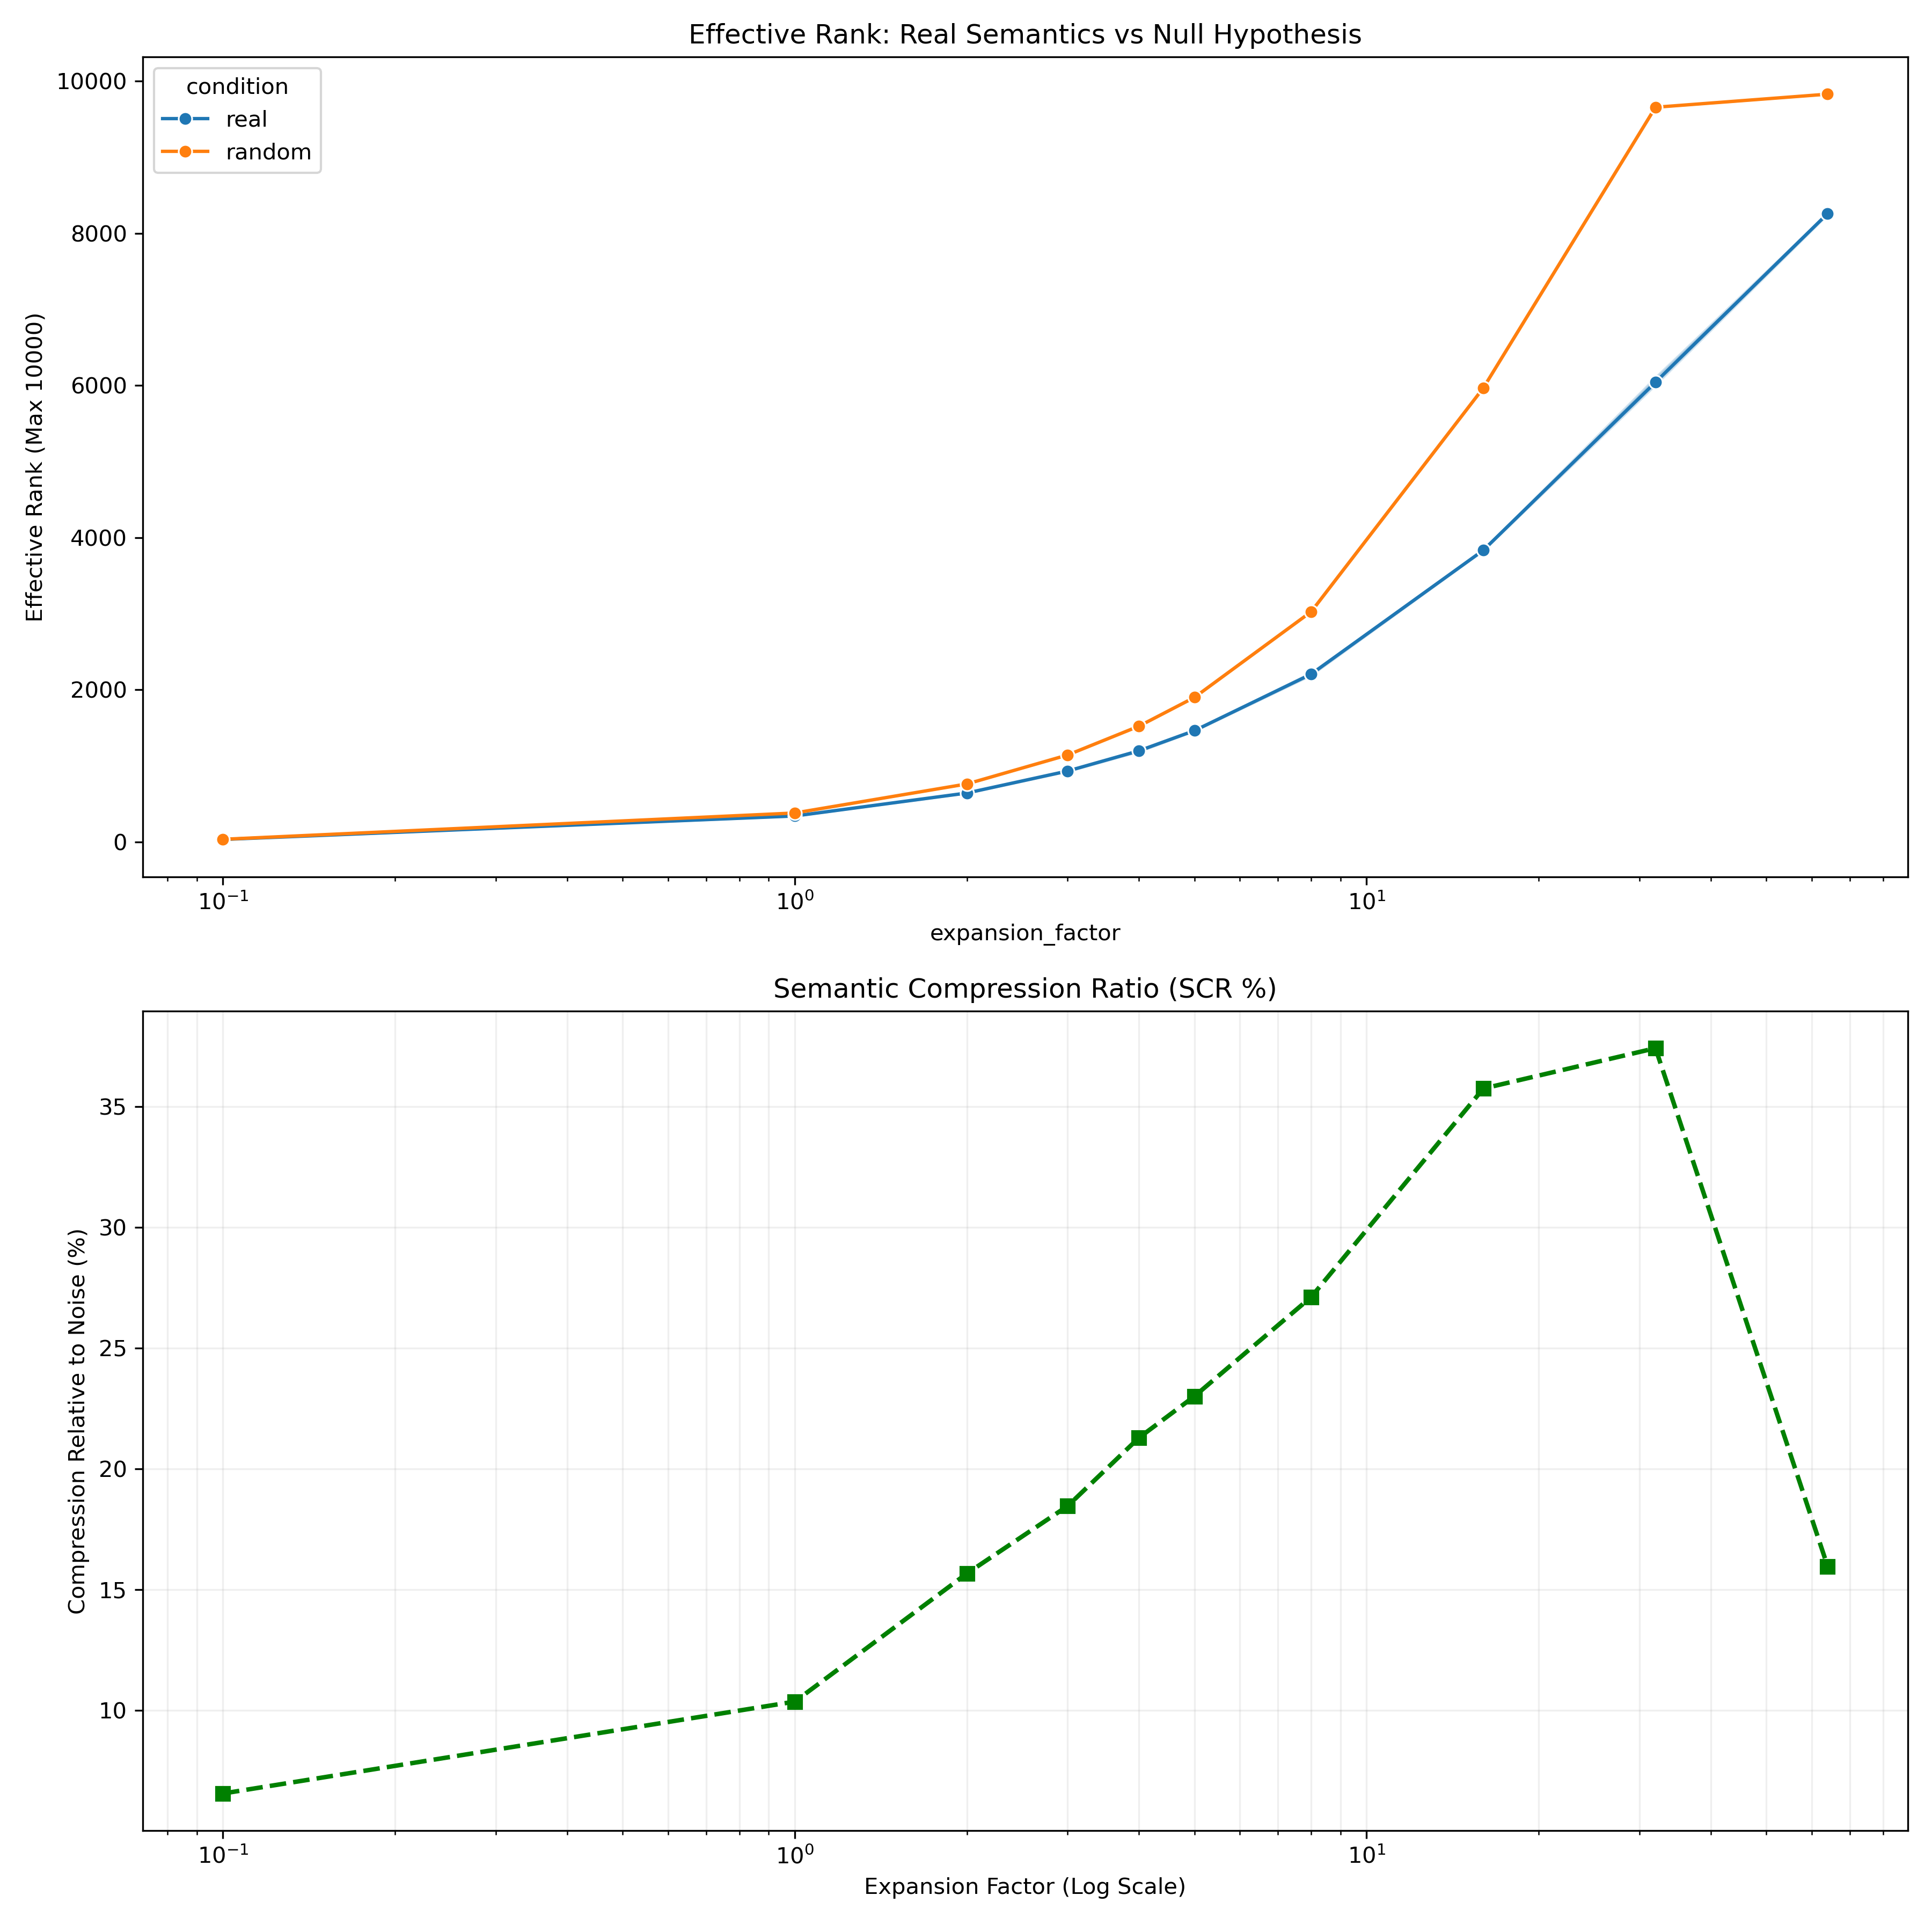
\includegraphics[width=\textwidth]{pictures/cap6/erank_ds11_ksing10000_ksparse16_analysis_1.png}
    \caption{Effective Rank in funzione dell'expansion factor, con limite a 10.000 autovalori. \textbf{Sopra}: confronto tra dati reali (blu) e ipotesi nulla (arancione). Il plateau oltre $\rho \approx 26$ è un artefatto del limite computazionale. \textbf{Sotto}: Semantic Compression Ratio. Il calo dopo il picco è dovuto alla saturazione di entrambe le curve al limite degli autovalori, non a una reale diminuzione della compressione semantica.}
    \label{fig:er_10000}
\end{figure}

La Figura~\ref{fig:er_40000} mostra i risultati con limite esteso a 40.000 autovalori. I risultati sono qualitativamente diversi:

\begin{itemize}
    \item Il plateau scompare: l'Effective Rank continua a crescere per entrambe le condizioni
    \item Il gap tra dati reali e casuali \textbf{aumenta} con l'expansion factor
    \item Il Semantic Compression Ratio cresce \textbf{monotonicamente}, raggiungendo il 59,9\% per $\rho = 64$
\end{itemize}

\begin{figure}[htbp]
    \centering
    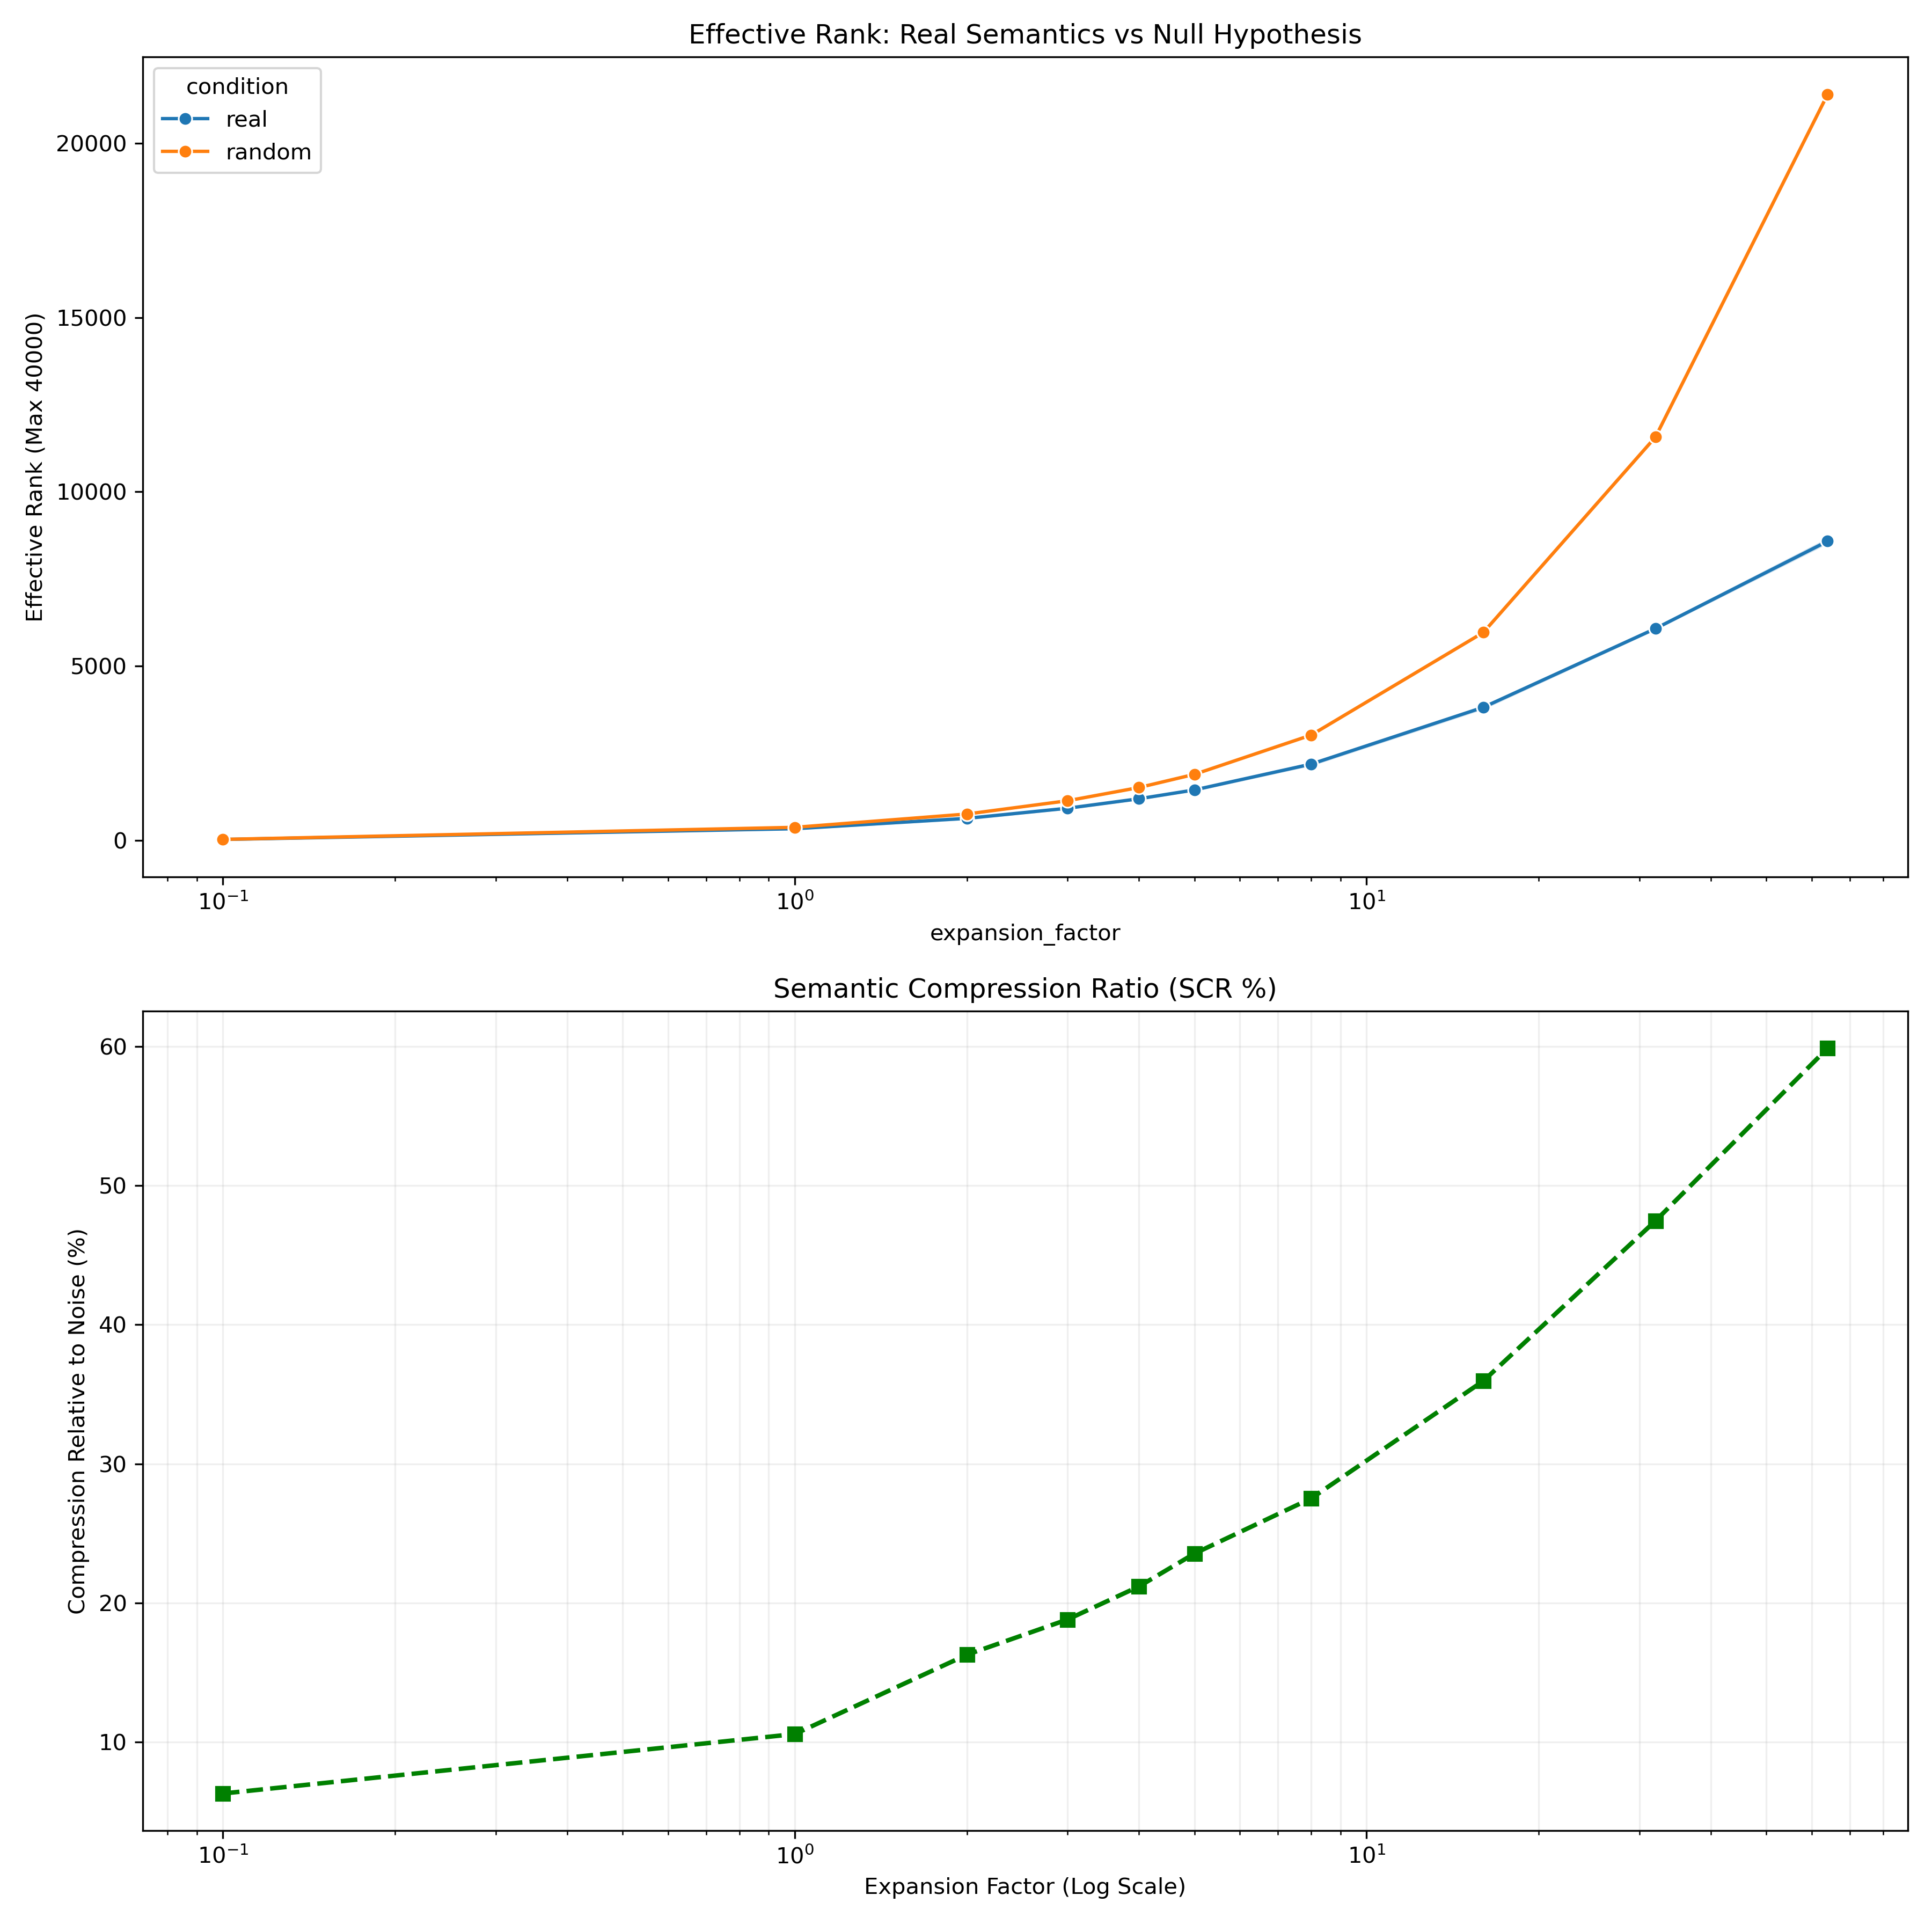
\includegraphics[width=\textwidth]{pictures/cap6/erank_ds11_ksing40000_ksparse16_analysis_1.png}
    \caption{Effective Rank in funzione dell'expansion factor, con limite a 40.000 autovalori. \textbf{Sopra}: senza il limite artificiale, l'Effective Rank continua a crescere. Il gap tra le due condizioni aumenta progressivamente. \textbf{Sotto}: il Semantic Compression Ratio cresce monotonicamente fino al 59,9\%, indicando che la struttura semantica comprime sempre più le rappresentazioni all'aumentare della capacità.}
    \label{fig:er_40000}
\end{figure}

\subsubsection{Interpretazione dei risultati}
\label{subsubsec:er_interpretation}
I risultati dell'analisi dell'Effective Rank supportano due conclusioni principali.
\paragraph{La struttura semantica comprime le rappresentazioni.}
Il gap persistente tra dati reali e casuali, quantificato dal Semantic Compression Ratio, dimostra che i dati linguistici reali occupano una varietà di dimensionalità inferiore rispetto a dati casuali nella stessa configurazione architettonica. Questa compressione non è un artefatto del vincolo Top-K (presente in entrambe le condizioni), ma riflette le correlazioni intrinseche del dominio semantico: concetti correlati (febbre $\leftrightarrow$ infezione, gradiente $\leftrightarrow$ ottimizzazione) tendono a co-attivarsi, riducendo la dimensionalità effettiva.
\paragraph{L'SCR crescente è consistente con il feature splitting.}
L'aumento monotono del Semantic Compression Ratio con l'expansion factor (Figura~\ref{fig:er_40000}) è coerente con il fenomeno del feature splitting descritto nel Paragrafo~\ref{subsubsec:feature_splitting}. All'aumentare della capacità, le feature generali si scindono in sotto-feature più specifiche. Queste sotto-feature, pur essendo distinte, rimangono tuttavia \textit{correlate}: appartengono alla stessa famiglia semantica, si attivano su sottoinsiemi sovrapposti di documenti, e le loro direzioni decoder formano angoli non ortogonali.
In altri termini: il feature splitting aumenta il numero di feature \textit{nominali} ($n$), ma non aumenta proporzionalmente la dimensionalità \textit{effettiva} (ER). Le nuove feature emergenti non sono indipendenti dalle precedenti, bensì loro specializzazioni. Questo spiega perché l'SCR \textit{aumenta} con l'expansion factor: più feature, ma meno indipendenza relativa.
\begin{notebox}
\textbf{Il paradosso della capacità, rivisitato}\\[0.5em]
Nel Paragrafo~\ref{sec:04_disentanglement} è stato introdotto il paradosso della capacità: come può un modello come BERT~\parencite{devlin2018bert} rappresentare decine di migliaia di concetti con soli 768 neuroni?
L'analisi dell'Effective Rank suggerisce una risposta parziale: quei concetti non sono \textit{indipendenti}. La struttura semantica del linguaggio, vale a dire le relazioni tassonomiche, le co-occorrenze, le analogie, introduce correlazioni che permettono di comprimere molti concetti in poche dimensioni effettive.
Lo Sparse Autoencoder non elimina queste correlazioni: le rende \textit{esplicite}, mappandole in famiglie e gerarchie interpretabili.
\end{notebox}